\documentclass{article}

\usepackage{subfigure}
\usepackage{graphicx}
\usepackage{xepersian}
\settextfont{Yas}
\setlatintextfont{Times New Roman}
\setmathdigitfont{Yas}
\renewcommand{\baselinestretch}{1.3}
\title{گزارش کار تمرین دوم-طبقه بندی متن}
\author{محمد لشکری ۴۰۰۱۱۲۰۸۷}

\begin{document}
	\maketitle
	\section{پیش‌پردازش دادگان}
	در تابع 
	\lr{clean\textunderscore text()}
	تمامی کاراکتر‌ها به‌جز نقطه، علامت سوال، حروف فارسی، اعداد و فاصله حذف شدند. همچنین اعداد با کاراکتر N جایگزین شدند و کاراکتر 
	\lr{$\backslash$xa0}
	نیز از دادگان حذف شده ‌است. 
	
	تابع 
	\lr{count\textunderscore words()}
	تعداد تکرار هر توکن منحصر به فرد را در دیکشنری 
	\lr{frequencies}
	ذخیره می‌کند و بعد از مرتب‌سازی، ۲۰۰ توکن پرتکرار را در فایل 
	\lr{frequent.txt}
	ذخیره می‌کند. سپس تعداد توکن‌ها چاپ می‌شود. تعداد توکن‌های منحصر به فرد و تعداد کل توکن‌های مجموعه آموزشی به ترتیب
	 $ 437,183 $
	  و
	   $ 32,058,511 $
	     و برای مجموعه آزمایشی به ترتیب
	     $ 143,365 $
	       و
	       $ 5,794,586 $
	        است.
	لازم به ذکر است نمونه هایی که برچسب با نام category داشتند که تعداد آنها ۸ بوده از دادگان حذف شده‌اند. 
	سه نمونه از نتاظر‌های انجام شده در جدول \ref{table1} قابل مشاهده است.
	\begin{table}[h]
		\begin{center}
			\begin{tabular}{|c|c|}
				\hline
				کلمه & اندیس \\
				\hline
				\hline
				گفت & ۲۰ \\
				هم &  ۳۰ \\
				مردم & ۵۰ \\
				\hline
			\end{tabular}
		\caption{نمونه‌های تناظرهای انجام‌شده}
		\label{table1}
		\end{center}
	\end{table}
	\begin{figure}[h]
		\begin{center}
			\includegraphics[height=10cm, width=10cm]{plot.png}
			\caption{توزیع دادگان آموزشی}
			\label{plot}
		\end{center}
	\end{figure}
	\newpage
	\section{طبقه‌بندی کننده بیز ساده}
	در تابع 
	\lr{count\textunderscore word \textunderscore per\textunderscore class()}
	یک دیکشنری به نام 
	\lr{count\textunderscore per\textunderscore class\textunderscore dict}
	تعداد تکرار هر کلمه در هر کلاس را نگهداری می‌کند. دیکشنری 
	\lr{count\textunderscore allwords\textunderscore per\textunderscore class}
	تعداد تکرار همه کلمات موجود در هر کلاس را نگهداری می‌کند. لگاریتم احتمال‌های 
	\lr{prior}
	نیز در این تابع محاسبه و در لیست 
	\lr{log\textunderscore prior\textunderscore list}
	ذخیره می‌شود و در تابع 
	\lr{calculate\textunderscore log\textunderscore prior()}
	فقط مقدار آن بازگردانده می‌شود تا مدل کاراتر
	\LTRfootnote{More efficient}
	 باشد.
	 \subsection{ارزیابی}
	 نتایج حاصل شده برای مجموعه‌های آموزشی و آزمایشی در دو جدول زیر قابل مشاهده است:
	 
	 \begin{figure}[h]
	 	\begin{center}
	 		\subfigure[نتایج دادگان آزمایشی]{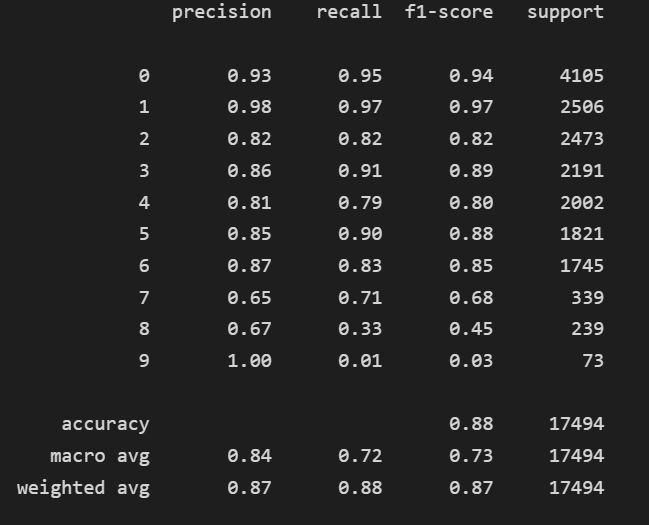
\includegraphics[height=5cm, width=5cm]{result-test-set.png}}
	 		\hspace*{0.2cm}
	 		\subfigure[نتایج دادگان آموزشی]{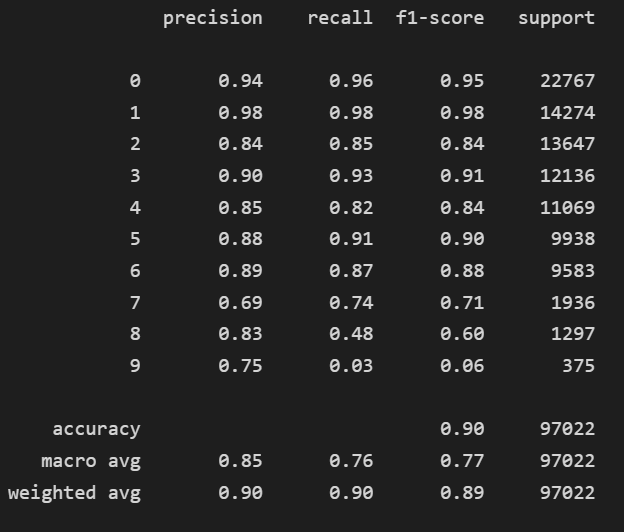
\includegraphics[height=5cm, width=5cm]{result-training-set.png}}
	 	\end{center}
	 \end{figure}
 	از آنجا که توزیع داداگان متوازن نیست، بهترین معیار ارزیابی میانگین ماکروی
 	 \lr{F1}
 	  است. \lr{F1} دادگان آمورشی به \lr{F1} نزدیک است که نشان می‌دهد مدل بیش از حد آمورش ندیده است. مقادیر recall برای سه کلاس با کمترین فراوانی از سایر کلاس‌ها کمتر است که نشان می‌دهد مدل به سمت کلاس‌های با فراوانی بالاتر bias شده است.
 	  
\end{document}